\documentclass[11pt]{article}
\usepackage[utf8]{inputenc}
\usepackage{geometry}
\usepackage{graphicx}
\usepackage{hyperref}
\usepackage{amsmath}
\usepackage{listings}
\usepackage{float}
\usepackage{subcaption}
\usepackage{algorithm}
\usepackage{algpseudocode}
\usepackage{booktabs} % For prettier tables
\usepackage{siunitx}
\usepackage{amssymb}
\usepackage{subcaption}

% Set page margins
\geometry{a4paper, margin=1in}

% Set up code listing style
\lstset{
    basicstyle=\ttfamily,
    commentstyle=\colour{gray},
    keywordstyle=\colour{blue},
    stringstyle=\colour{red},
    showstringspaces=false,
    captionpos=b
}

\title{Image Analysis Coursework}
\author{Vishal Jain}
\date{\today}

\begin{document}
\section{Question 1 - Image Segmentation}
This question details the segmentation algorithms used to segment the required sections of the lung ct image, the noisy flowers and the coin images.
\subsection{Part A: Lung CT Image Segmentation}
This section details the segmentation algorithm of the Lung CT image shown in Figure \ref{fig:lung_ct_image}. The region to be segmented is the lung area, including all the nodules and tissue within. The image is taken from the LIDC-IDRI dataset \cite{lidc_idri}.
\begin{figure}[H]
    \centering
    \includegraphics[width=0.5\textwidth]{../data/CT.png}
    \caption{Lung CT image from the LIDC-IDRI dataset.}
    \label{fig:lung_ct_image}
\end{figure}

\subsubsection{Image Characteristics}
The image shows a high contrast between the lungs and surrounding non lung tissue. This observation motivates a threshold based approach to segment the lung area. The nodules and tissue in the intra lung regions are of a much higher intensity than the lung tissue, as such it is appropriate supplement the thresholding step with additional morphological operations.

\subsubsection{Assumptions}
The algorithm assumes that after binarising the image via thresholding, the background makes up the largest connected component, with the left and right lungs being the next two largest. The algorithm also assumes that the nodules and tissue within the lung regions are fully enclosed and do not touch the border of the lung regions.

\subsubsection{Segmentation Algorithm}
The segmentation algorithm for the lung CT image is as follows:
\begin{itemize}
    \item \textbf{Binarise Image via Otsu Thresholding:} The image is thresholded using Otsu's threshold. This is a global thresholding method that maximises the inter-class variance of foreground and background. 
    \item \textbf{Connected Component Analysis:} The binary image is inverted to make the lung and background regions the foreground. The connected components of the inverted image are labelled using 8-connectivity. The second and third largest connected components are selected to recover the left and right lung regions. The connected components are selected based on their area. 
    \item \textbf{Binary Hole Filling} To recover the nodules and tissue within the lung regions, binary hole filling is performed. The algorithm fills holes in a binary image by inverting the image, labelling connected regions, and converting regions not connected to the border from background to foreground.
    \end{itemize}
    \begin{figure}[H]
        \centering
        \begin{subfigure}{.3\textwidth}
            \centering
            \includegraphics[width=\linewidth]{figs/q1a_binary.png}  % Replace with your image file
            \caption{}
            \label{fig:otsu_threshold}
        \end{subfigure}%
        \begin{subfigure}{.3\textwidth}
            \centering
            \includegraphics[width=\linewidth]{figs/q1a_largest_connected_components.png}  % Replace with your image file
            \caption{}
            \label{fig:connected_components}
        \end{subfigure}%
        \begin{subfigure}{.3\textwidth}
            \centering
            \includegraphics[width=\linewidth]{figs/q1a_filled_holes.png}  % Replace with your image file
            \caption{}
            \label{fig:filled_holes}
        \end{subfigure}
        \label{fig:segmentation_steps}
    \caption{Key steps in the segmentation of the lung CT image: (a) Binarisation using Otsu's threshold, (b) Mask inversion and selection of lung regions via connected component analysis, (c) Recovery of internal structures through binary hole filling.}
    \end{figure}
Note, this segmentation algorithm was also implemented from scratch. Relevant code can be found in \texttt{src/q1a\_from\_scratch.py} and \texttt{src/from\_scratch\_seg\_funcs.py}.
\subsubsection{Results}
The final segmentation of the lung CT image is shown in Figure \ref{fig:lung_ct_image} The segmentation clearly captures the relevant lung regions and all the nodules and tissues within.
\begin{figure}[H]
    \centering
    \includegraphics[width=0.4\textwidth]{figs/q1a.png}
    \caption{Final segmentation of the lung CT image.}
    \label{fig:lung_ct_segmentation}
\end{figure}

\subsubsection{Discussion}
Figure \ref{fig:q1a_ambiguity} shows a potential ambiguous region in the segmentation. This region was segmented due to having a similar intensity as the lung tissue and being connected to lung tissue post Otsu thresholding. However, as this region could not be clearly identified as non lung tissue without additional context, it was kept in the final segmentation. This also highlights the limitations of thresholding based segmentation methods in identifying regions that are not clearly defined by intensity.
\begin{figure}[H]
    \centering
    \begin{subfigure}{.4\textwidth}
        \centering
        \includegraphics[width=\linewidth]{figs/q1a_seg_w_bbox.png}  % Replace with your image file
        \caption{}
        \label{fig:q1a_seg_w_bbox}
    \end{subfigure}%
    \begin{subfigure}{.4\textwidth}
        \centering
        \includegraphics[width=\linewidth]{figs/q1a_zoomed_region.png}  % Replace with your image file
        \caption{}
        \label{fig:q1a_zoomed_region}
    \end{subfigure}%
    \caption{Ambiguous region in the segmentation: (a) Segmentation with bounding box around the ambiguous region, (b) Zoomed in view of the ambiguous region.}
    \label{fig:q1a_ambiguity}
\end{figure}

\subsection{Part B: Noisy Flowers Image Segmentation}
This section details the segmentation algorithm of the noisy flowers image shown in Figure \ref{fig:flowers_image}. The region to be segmented are all the purple flower heads in the image.

\begin{figure}[H]
    \centering
    \includegraphics[width=0.8\textwidth]{../data/noisy_flower.jpg}
    \caption{Noisy Flowers image.}
    \label{fig:flowers_image}
\end{figure}

\subsubsection{Image Characteristics}
The image features a type of noise that is typical to gaussian degradations. This was confirmed by applying a gaussian filter to each of the colour channels seperately in the image and observing that nearby pixel colours were more. This effect is shown in Figure \ref{fig:gaussian_noise_evidence}. 
\begin{figure}[H]
    \centering
    \begin{subfigure}{.4\textwidth}
        \centering
        \includegraphics[width=\linewidth]{figs/q1b_patch.png}  % Replace with your image file
        \caption{}
        \label{fig:flower_patch}
    \end{subfigure}%
    \begin{subfigure}{.4\textwidth}
        \centering
        \includegraphics[width=\linewidth]{figs/q1b_gauss_blurred_patch.png}  % Replace with your image file
        \caption{}
        \label{fig:gaussian_filtered_flower_patch}
    \end{subfigure}%
    \caption{Effect of Gaussian filtering on the colour channels of the noisy flowers image: (a) Cropped region of the noisy flowers image, (b) Cropped region after applying a Gaussian filter with standard deviation 1.}
    \label{fig:gaussian_noise_evidence}
\end{figure}
The purple flowers in \ref{fig:flowers_image}, except for the ones clearly in the foreground, are all roughly of the same shade of purple. There are two batches of purple flowers in the image, one large group down the middle and another smaller group along the upper left corner of the image. The purple flowers in the foreground have shadows on them making the bottom half of the flower darker than the top half. Due to the general uniformity in colours of the flower after denoising, a clustering type algorithm is appropriate for this image.

\subsubsection{Assumptions}
The main assumption made by this algorithm is in choosing the number of clusters. The number of clusters is chosen to be 5, which is chosen based on the number of distinct colours in the image. The green grass and stems, the orange flower heads, the purple flower heads, the white flower heads and the red flower heads.

\subsubsection{Segmentation Algorithm}
The segmentation algorithm for the noisy flowers image is as follows:
\begin{itemize}
    \item \textbf{Bilateral Gaussian Filtering:} First the image was denoised using a bilateral filter \cite{710815}. This filter was chosen for its ability to denoise while considering both spatial proximity and colour similarity, ideal for preserving flower head edges. A spatial standard deviation of 15 was chosen to allow for smoothing across the entire flower head regions, while a colour standard deviation of 1 ensures edge sharpness by only blending similarly coloured pixels. This approach effectively reduces noise without blurring distinct colour boundaries.
    \item \textbf{Conversion from RGB to LAB colour Space:} The image is converted from RGB to LAB colour space, which better approximates human vision by separating colour and luminance. This space enhances clustering accuracy because Euclidean distances more closely reflect perceptual differences, making it ideal for grouping similar colours like purple flower heads.
    \item \textbf{K-Means Clustering:} K-means clustering is applied to the LAB image. The number of clusters is chosen to be 5, based on the number of distinct colours in the image. The image is then segmented by assigning each pixel to the cluster with the closest centroid.
    \item \textbf{Select Purple Pixels} The cluster centre closest to the the LAB value of purple is chosen to be the desired cluster to represent the foreground. The image is binarised by setting all pixels not in this cluster to 0 and all pixels in this cluster to 1.
    \item \textbf{Denoise Segmentation via Morphological Opening} To remove small-scale noise from the mask while retaining the shape and size of the main flower heads, a morphological opening operation is applied. 
    \item \textbf{Remove Small Connected Components:} Finally to remove any left over noise, all connected components with an area less than 100 pixels are removed. The previous morphological opening step ensures the required thresholding does not remove any of the main flower heads.
\end{itemize}
\begin{figure}[H]
    \centering
    \begin{subfigure}{.45\textwidth}  % Adjusted to fit two figures per row
        \centering
        \includegraphics[width=\linewidth]{figs/q1b_denoised.png}
        \caption{}
        \label{fig:denoised_flowers}
    \end{subfigure}%
    \begin{subfigure}{.45\textwidth}  % Adjusted to fit two figures per row
        \centering
        \includegraphics[width=\linewidth]{figs/q1b_kmeans_mask.png}
        \caption{}
        \label{fig:kmeans_mask_flowers}
    \end{subfigure}
    \begin{subfigure}{.45\textwidth}  % New row, first column
        \centering
        \includegraphics[width=\linewidth]{figs/q1b_kmeans_mask_post_opening.png}
        \caption{}
        \label{fig:kmeans_mask_post_opening_flowers}
    \end{subfigure}%
    \begin{subfigure}{.45\textwidth}  % New row, second column
        \centering
        \includegraphics[width=\linewidth]{figs/q1b_mask_post_cnc_removal.png}
        \caption{}
        \label{fig:cnc_threshold_flowers}
    \end{subfigure}%
    \caption{Segmentation process for the noisy flowers image: (a) Image after denoising with a bilateral filtering, showing reduced colour noise while preserving edge details. (b) Result of applying K-means clustering to segment purple pixels. (c) Segmentation mask post morphological opening, illustrating reduced noise in the segmentation. (d) Final segmentation after removing small connected components, highlighting the refined segmentation of flower regions.}
    \label{fig:q1b_segmentation_steps}
\end{figure}

\subsubsection{Results}
The final segmentation of the noisy flowers image is shown in Figure \ref{fig:q1b_final_mask}. The segmentation clearly captures most of the purple flower heads in the main central bunch. It also captures some in the smaller bunch in the upper left corner. It is able to distinguish between the colours effectively, with some of the orange and red flowers in the purple group being excluded from the segmentation quite effectively as seen in figure \ref{fig:flowers_seg_zoomed}.

\begin{figure}[H]
    \centering
    \includegraphics[width=0.8\textwidth]{figs/q1b_final_mask.png}
    \caption{Final segmentation of the noisy flowers image.}
    \label{fig:q1b_final_mask}
\end{figure}

% TODO: Think of a better colouring scheme for the bounding boxes, white is washing out the image.
\begin{figure}[H]
    \centering
    \begin{subfigure}[c]{.6\textwidth}  % Centered subfigure on the left
        \centering
        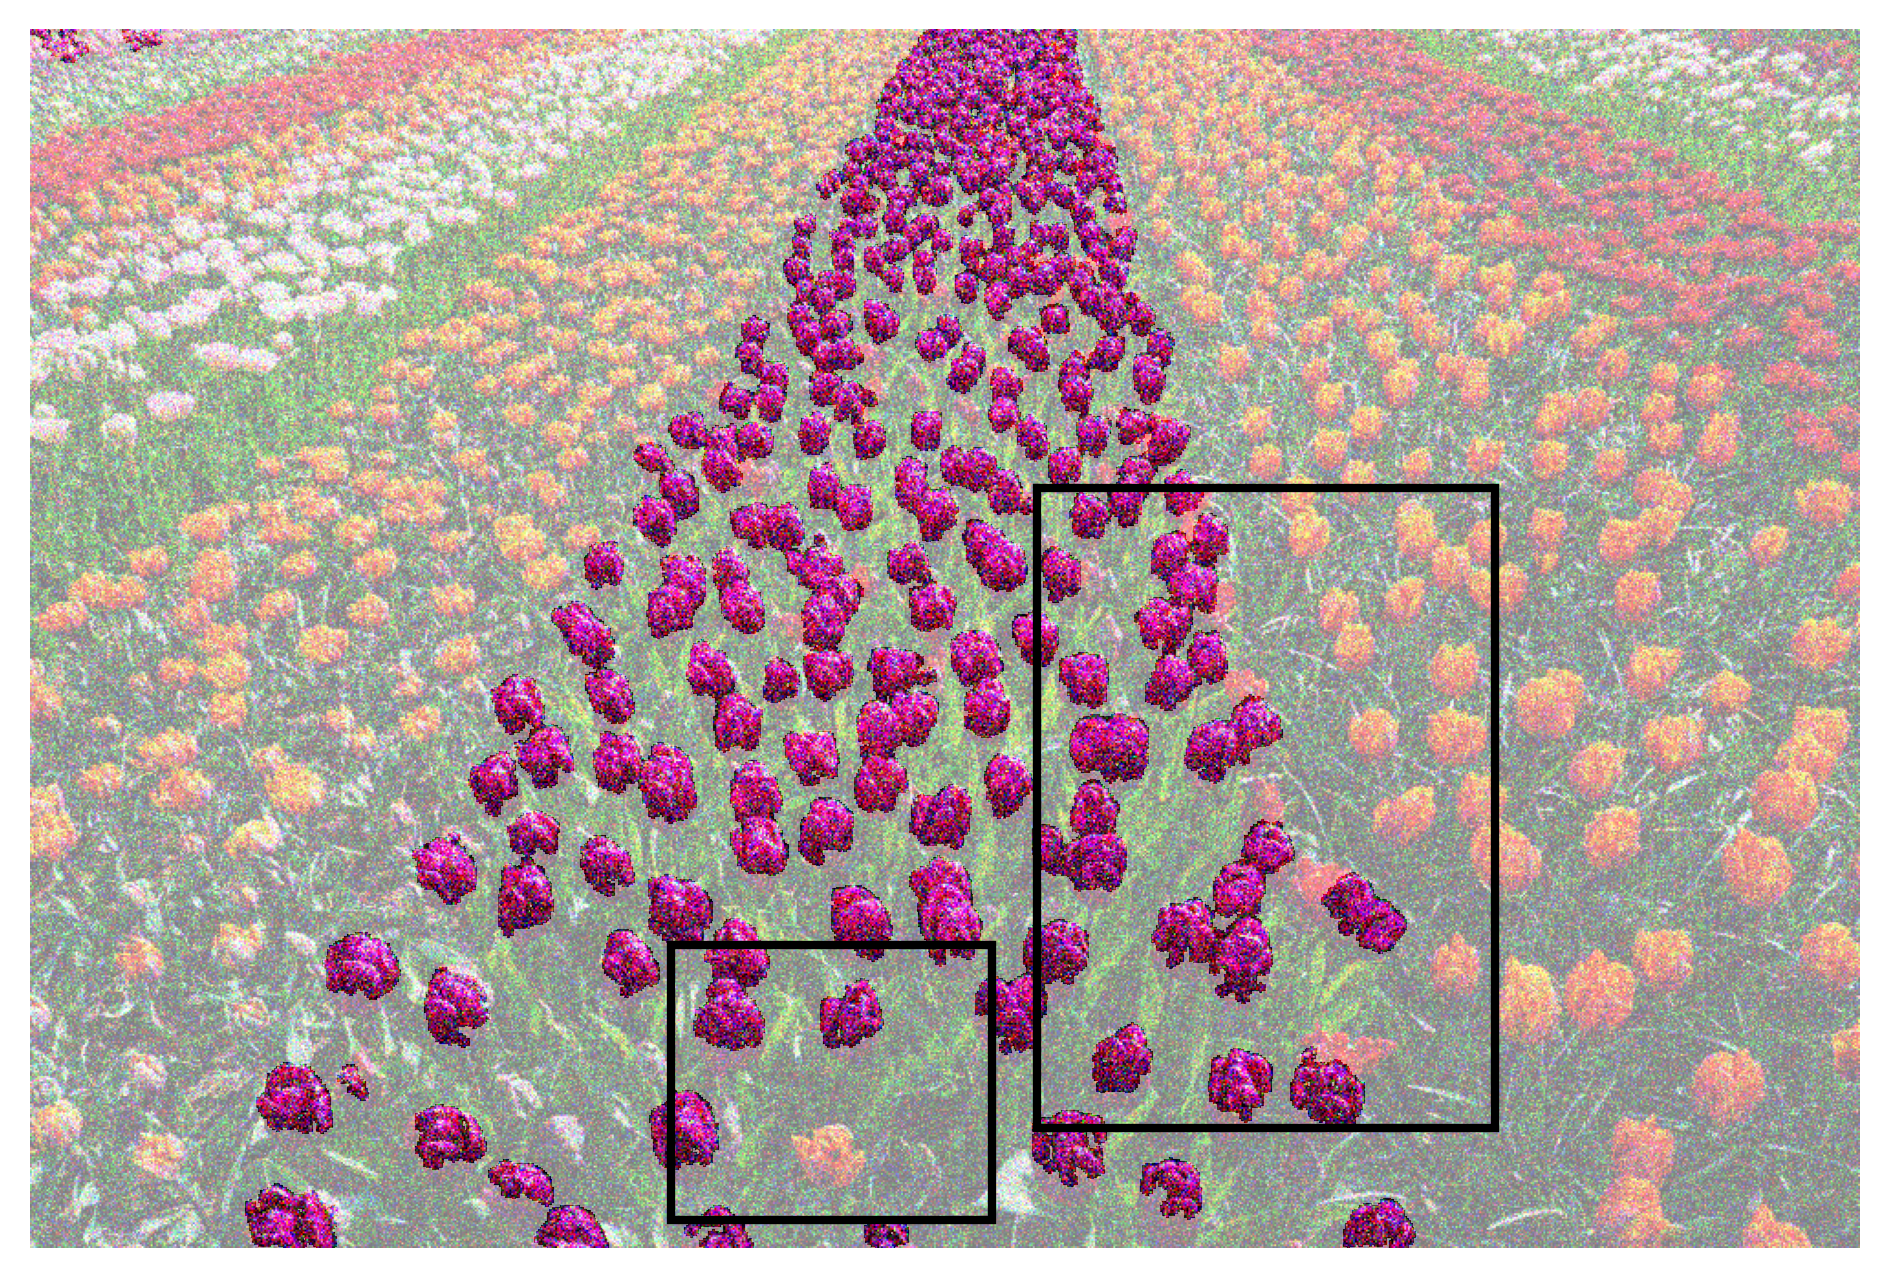
\includegraphics[width=\linewidth]{figs/q1b_seg_w_good_bbox.png}
        \caption{}  % Caption for the left subfigure
        \label{fig:q1b_zoomed}
    \end{subfigure}%
    \begin{minipage}[c]{.35\textwidth}  % Centered minipage for the right subfigures
        \begin{subfigure}{\textwidth}
            \centering
            \includegraphics[width=\linewidth]{figs/q1b_zoomed_region1.png}
            \caption{}  % Caption for the upper right subfigure
            \label{fig:q1b_zoomed_bad}
        \end{subfigure}\\[1ex]  % Add some space between the subfigures
        \begin{subfigure}{\textwidth}
            \centering
            \includegraphics[width=\linewidth]{figs/q1b_zoomed_region2.png}
            \caption{}  % Caption for the lower right subfigure
            \label{fig:q1b_zoomed_bad2}
        \end{subfigure}
    \end{minipage}
    \caption{Zoomed in view of the segmentation: (a) Segmentation with bounding boxs around regions of interest where the segmentation has performed well, (b) Zoomed in view of the segmentation showing the exclusion of orange flower from the purple group, (c) Zoomed in view of the segmentation showing the exclusion of orange and red flowers that are occluded by flowers from the purple group.}
    \label{fig:flowers_seg_zoomed}
\end{figure}

\subsubsection{Discussion}
The main challenge in this segmentation is the segmentation of the purple flower heads that are in the foreground (closest to the camera). These flower heads have shadows on them, making the bottom half of the flower darker than the top half, making them difficult to fully segment with the current approach. An example such case is shown in figure \ref{fig:q1b_seg_lim}. This highlights the limitations of a segmentation algorithm which segments purely on colour. A potential improvement to this algorithm would be to consider spatial shape based information to better segment these flower heads or make use of more sophisticated pre-processing to remove the shadows.
% TODO: Make it clearer where the seg is failing, right now the masks are not showing in the zoomed regions so not obvious
\begin{figure}[H]
    \centering
    \begin{subfigure}{.8\textwidth}
        \centering
        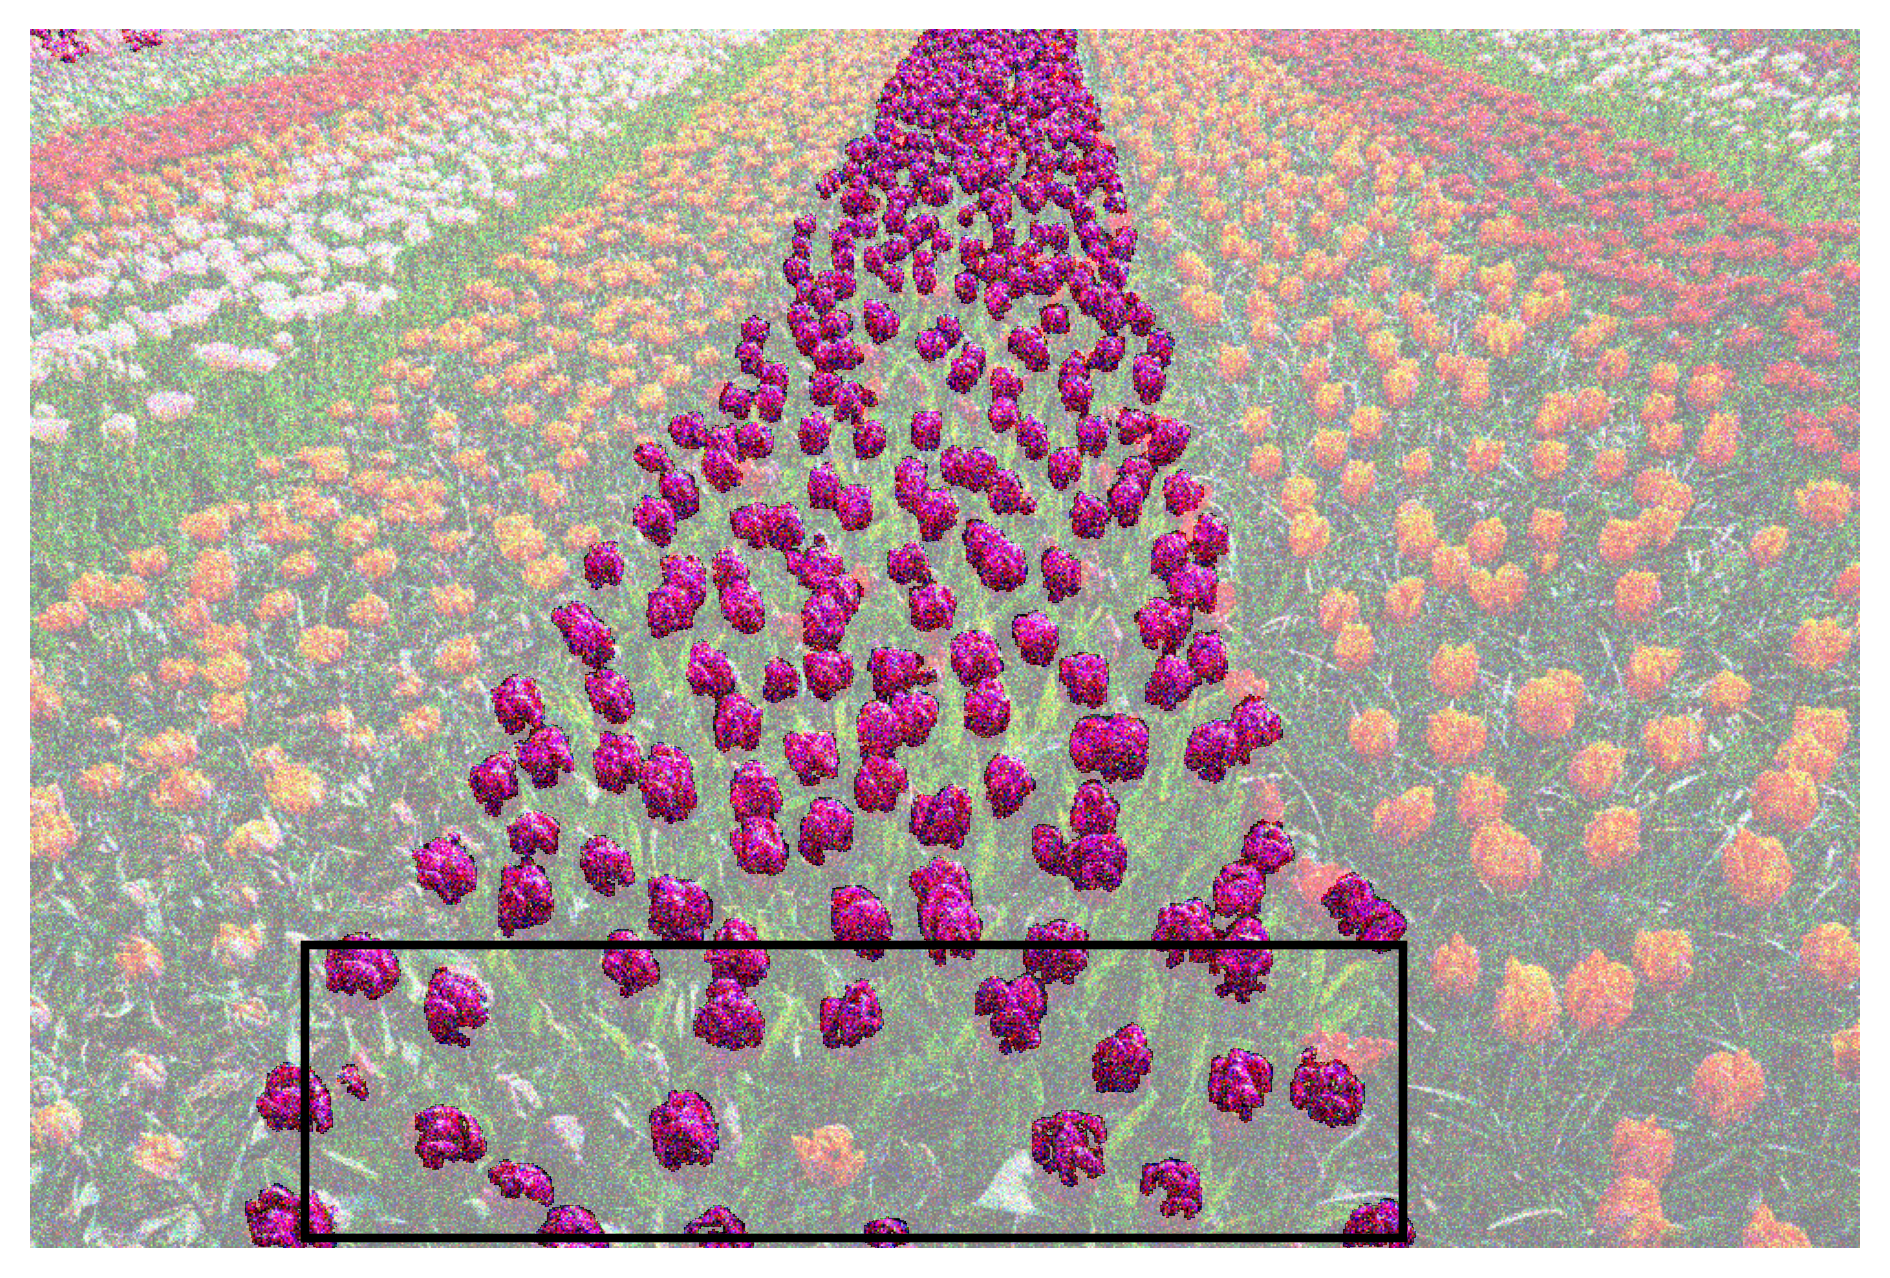
\includegraphics[width=\linewidth]{figs/q1b_seg_w_bad_bbox.png}
        \caption{}  % Optional: add a specific caption here if needed.
        \label{fig:q1b_bad_seg_w_bbox}
    \end{subfigure}\\ % Add a line break to stack the next subfigure below
    \begin{subfigure}{.8\textwidth}
        \centering
        \includegraphics[width=\linewidth]{figs/q1b_bad_zoomed_region.png}
        \caption{}  % Optional: add a specific caption here if needed.
        \label{fig:q1b_bad_zoom}
    \end{subfigure}
    \caption{Limitations in segmentation of noisy flowers image: (a) Full view of the image with poorly segmented areas highlighted in a bounding box, demonstrating where the algorithm fails to accurately segment due to shadows. (b) Close-up view of a poorly segmented area, showing flower heads which feature strong shadows, impacting segmentation accuracy.}
    \label{fig:q1b_seg_lim}
\end{figure}

\bibliographystyle{plain}  % Choose the style that suits your needs
\bibliography{references}  % The filename of the .bib file, without the extension
\end{document}